\section{Parsing}
\label{sec:parsing}
% GIACOMO

The parsing process is responsible to generate a DUDES from a question expressed in natural language. 
%
The parser takes in input a \textit{SLTAG grammar} and a \textit{question} expresed in english natural language, and generates the minimal \textit{DUDES} representing the semantic of the question.
%
The DUDES will be used, at the end, to generate a \textit{SPARQL query} that will be submitted to the ontology which the SLTAG grammar is aligned to.
%
The parser has been designed addressing the minimization of the search space, that is the most critical requirements to achieve better performance.
%
The previous requirement have been met with a parsing algorithm that is (i) deterministic (ii) greedy and (iii) principally focused on structural aspects of LTAGs.

The parsing process is carried out by two functional components: 
(i) the \texttt{Tokenizer}, which recognized in the sentence textual patterns that can be traced back to ESLTAGs within the grammar, and sequentially emit them as tokens, and 
(ii) the \texttt{Parser} itself, which consumes these tokens to generate the final DUDES.

In Section~\ref{sec:parsing-tokenizer} and Section~\ref{sec:parsing-parser} we describe and motivate the architectural choices and the pseudocode of the \texttt{Tokenizer} and \texttt{Parser}, respectively.


\subsection{Tokenizer}
\label{sec:parsing-tokenizer}
The \texttt{Tokenizer} is the component responsible of partitioning the sentence $S$ in a ordered sequence of textual patterns $\{\pi\}$, where each one can be traced back to one or more ESLTAGs within the grammar $G$ it is associated to. 
%
In Figure~\ref{fig:tokenizer-sample} we show a sample of the tokenization process.
%
Every time the \texttt{Tokenizer} is invoked on $S$ with $G$, it looks in $S$ for textit{the longest regular expression associated in $G$ with at least one SLTAG}. Once the regular expression has been matched, it emits a \texttt{Token} $t$, that is an element defined as follows:

\begin{equation}
\label{eqn:token}
t:=(regexp,i,candidates)
\end{equation}

where
$regexp$ is the regular expression matched in the substring of $S$ starting at position $i$, and
$candidates$ is the list of SLTAG in $G$ associated with $regexp$.

\begin{figure}[tp]
	\centering
	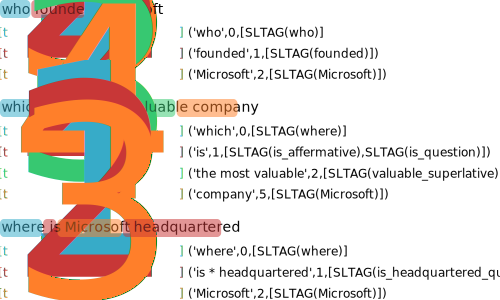
\includegraphics{./fig/tokenizer-sample}
	\caption{An example of the tokenization process.}
	\label{fig:tokenizer-sample}
\end{figure}

The \texttt{Tokenizer} is stateful component, hence it leverages convenient data structures to incapsulate its state.
%
The most important one is the \texttt{TokenizerBuffer}, that records which word in $S$ has been already tokenized and tokenizable, or not.

Given the sentence $S$, the \texttt{TokenizerBuffer} is a list of elements $be$ defined as follows:

\begin{equation}
\label{eqn:tokenizer-buffer-element}
	be:=(w, t_{1}, t_{2})
\end{equation}

where 
$w_{i}$ is the $i$-th word in $S$, 
$t_{1}$ is the boolean value that is true if $w_{i}$ has been already tokenized, and
$t_{2}$ is the boolean value tha is true if $w_{i}$ is tokenizable.


In Algorithm~\ref{alg:tokenizer} we show the pseudocode of the tokenization process.
%
The \texttt{Tokenizer} exposes a convenient API to iterate over tokens, that is clearly inspired to the well known API provided by Java generic iterators.

\begin{algorithm}[t]
	\SetKwProg{Fn}{Function}{}{}  
	
	\Fn{nextTokenizable()}{
	\For{$b\in buffer$}{
		\If{$b.tokenizable\; \& \; b.tokenized$}{
			\KwResult{$buffer.index(b)$}
		}
	}
	\KwResult{$-1$}
	}	

	\Fn{hasNext()}{
	\KwResult{$nextTokenizable() \neq -1$}
	}
	
	\Fn{next()} {
		$start \leftarrow nextTokenizable()$ \\
		\If{$start = -1$}{
			\KwResult{$NULL$}
		}
	
		$end \leftarrow start$ \\
		
		\While{$end < buffer.size$}{
			$elem \leftarrow buffer.get(end)$ \\
			\If{$elem.tokenized = False$}{
				$tmpRegexp.concat(elem.word)$ \\
			}
			$matchType \leftarrow grammar.matchMode(tmpRegexp)$ \\
			\If{$matchType = FULL$}{
				$candidates \leftarrow grammar.getAll(tmpRegexp)$ \\
				$regexp \leftarrow tmpRegexp$ \\
				$buffer.get(end).tokenized \leftarrow True$ \\
				\If{$returnFirstFull = True$}{
					break
				}
			}
			\ElseIf{$matchType = NONE$}{
				break
			}
			\ElseIf{$matchType = PART$}{
				$buffer.get(end).tokenized \leftarrow True$ \\
			}
			\ElseIf{$matchType = STAR$}{
				\If{$consuming = False$}{
					$consuming \leftarrow True$ \\
					$startConsuming \leftarrow end$ \\
				}
				\Else{
					\If{$end = buff.size - 1$}{
						$consuming \leftarrow False$ \\
						$end \leftarrow startConsuming - 1$ \\
						$returnFirstFull \leftarrow True$ \\
					}
				}
			}
		
			$end \leftarrow end + 1$ \\
		}
	
		\KwResult{$Token(regexp,pos,candidates)$}		
	}
	\caption{Pseudocode of the \texttt{Tokenizer} API.}
	\label{alg:tokenizer}
\end{algorithm}

Some functions in Algorithm~\ref{alg:tokenizer} have not been formally defined because they are pretty self-explanatory or have been partially introduced in previous sections.
For reader's sake, we briefly describe the most important ones here. 

\texttt{grammar.matchMode(entry)} matches the specified entry against the regular expressions associated with the SLTAGs in the grammar. 
%
The following match modes have are defined:
%
\begin{itemize}
	\item[FULL] the grammar contains a regular expression matching to entry, and no regular expression starting with entry. 
	For example, the entry \textit{'Microsoft'} matches is such way the grammar $\{who,founded,Microsoft\}$.
	
	\item[PART] the grammar contains no regular expression matching entry, but a regular expression starting with entry.
	For example, the entry \textit{'founders'} matches is such way the grammar $\{who,are,the,founders of,Microsoft\}$.
	
	\item[STAR] the grammar contains no regular expression matching entry, but a regular expression starting with entry and consuming the last art of it with the \textit{star-operator (*)}.
	For example, the entry \textit{'is'} matches is such way the grammar $\{where,is\;*\;headquartered,Microsoft\}$.

	\item[NONE] the grammar contains no regular expression matching entry in one of the previous modes.
	For example, the entry \textit{'Google'} matches is such way the grammar $\{who,founded,Microsoft\}$.
\end{itemize}

\texttt{grammar.getAll(entry)} retrieves from the grammar all the SLTAGs associated with a regular expression matching the entry\footnote{in \texttt{FULL} mode.}.


\subsection{Parser}
\label{sec:parsing-parser}

The \texttt{Parser} is a stateful component, hence it leverages convenient data structures to incapsulate its state.
%
The most important ones are the \texttt{ParserQueue} and the \texttt{ConflictList}.
%
The \texttt{ParserQueue} is made up of two parallell queues: one for the substitutions and one for the adjunctions. A SLTAG in enqueued when it is correctly parsed with no ambiguities, but its LTAG cannot be substituted nor adjuncted to the current working SLTAG.
%
The \texttt{ConflictList} collects conflicting SLTAG, distinguishing those marked as possibile candidates for substitution and possible candidates for adjunction. In particular, it associates each conflicting element with metadata about the region of text it arose from, as to reduce the search space for conflicts resolution.

In Algorithm~\ref{alg:parser} we show the pseudocode of the parsing process.
%
The \texttt{Parser} exposes a very simple API, made uo of only one function.

\begin{algorithm}[t]
\SetKwProg{Fn}{Function}{}{}  

\Fn{receive (x,y,w)} {
	
	\If{$(x,y)\in E(G)$}{
		updateLink(x,y,w) \\
		$U \leftarrow update(x) \cup update(y)$ \\
		\For{$u\in U$}{
			emitHidden(u)\;
		}
	}
	
	\ElseIf{$x\in V(G) \land y\in V(G)$}{
		addLink(x,y,w) \\
		$U \leftarrow update(x) \cup update(y)$ \\
		\For{$u\in U$}{
			emitHidden(u)\;
			emitPotential(u)\;
		}
	}
	
	\ElseIf{$x\in V(G) \land y\notin V(G)$}{
		addLink(x,y,w) \\
		$U \leftarrow update(y)$ \\
		\For{$u\in U$}{
			emitHidden(u)\;
			emitPotential(u)\;
		}
	}
	
	\ElseIf{$x\notin V(G) \land y\in V(G)$}{
		addLink(x,y,w) \\
		$U \leftarrow update(x)$ \\
		\For{$u\in U$}{
			emitHidden(u)\;
			emitPotential(u)\;
		}
	}  
	
	\Else{
		addLink(x,y,w)
	}
}

\Fn{update (x)}{
	$N \leftarrow Neighbors(x)$ \\
	$U \leftarrow \emptyset$ \\
	\For{$y\in N$}{
		\If{$(x,y)\notin E(G)$}{
			$U \leftarrow U \cup \{(x,y)\}$
		}
	}
	\For{$z\in N$}{
		\If{$(x,z)\notin E(G) \land z\neq y$}{
			$U \leftarrow U \cup \{(y,z)\}$
		}
	}
	\KwResult{$U$}
}
\caption{Pseudocode of the \texttt{Parser} API.}
\label{alg:parser}
\end{algorithm}

Some functions in Algorithm~\ref{alg:parser} have not been formally defined because they are pretty self-explanatory or have been partially introduced in previous sections.
For reader's sake, we briefly describe the most important ones here.  \texttt{emitHidden(u)} lets . . .